% !TEX TS-program = pdflatex
% !TEX encoding = UTF-8 Unicode

% This is a simple template for a LaTeX document using the "article" class.
% See "book", "report", "letter" for other types of document.

\documentclass[10pt,twocolumn]{article}

\usepackage[utf8]{inputenc} % set input encoding (not needed with XeLaTeX)
\usepackage{graphicx}
\usepackage{listings} 
\usepackage{xcolor,colortbl}
\usepackage[section]{placeins}
\usepackage{amsthm}
\usepackage{mathtools}
\graphicspath{ {images/} }

%%% Examples of Article customizations
% These packages are optional, depending whether you want the features they provide.
% See the LaTeX Companion or other references for full information.

%%% PAGE DIMENSIONS
\usepackage{geometry} % to change the page dimensions
\geometry{a4paper} % or letterpaper (US) or a5paper or....
\geometry{margin=0.55in} % for example, change the margins to 2 inches all round
% \geometry{landscape} % set up the page for landscape
%   read geometry.pdf for detailed page layout information

\usepackage{graphicx} % support the \includegraphics command and options

% \usepackage[parfill]{parskip} % Activate to begin paragraphs with an empty line rather than an indent

%%% PACKAGES
\usepackage{booktabs} % for much better looking tables
\usepackage{array} % for better arrays (eg matrices) in maths
\usepackage{paralist} % very flexible & customisable lists (eg. enumerate/itemize, etc.)
\usepackage{verbatim} % adds environment for commenting out blocks of text & for better verbatim
\usepackage{subfig} % make it possible to include more than one captioned figure/table in a single float
\usepackage{indentfirst}
\usepackage{amsfonts}
\usepackage{amssymb}
\usepackage{amsthm}
% These packages are all incorporated in the memoir class to one degree or another...

%%% HEADERS & FOOTERS
\usepackage{fancyhdr} % This should be set AFTER setting up the page geometry
\pagestyle{fancy} % options: empty , plain , fancy
\renewcommand{\headrulewidth}{0pt} % customise the layout...
\lhead{}\chead{}\rhead{}
\lfoot{}\cfoot{\thepage}\rfoot{}

%%% SECTION TITLE APPEARANCE
\usepackage{sectsty}
\allsectionsfont{\sffamily\mdseries\upshape} % (See the fntguide.pdf for font help)
% (This matches ConTeXt defaults)

%%% ToC (table of contents) APPEARANCE
\usepackage[nottoc,notlof,notlot]{tocbibind} % Put the bibliography in the ToC
\usepackage[titles,subfigure]{tocloft} % Alter the style of the Table of Contents
\renewcommand{\cftsecfont}{\rmfamily\mdseries\upshape}
\renewcommand{\cftsecpagefont}{\rmfamily\mdseries\upshape} % No bold!
\setlength{\parindent}{0.5cm} 

%%% END Article customizations

%%% The "real" document content comes below...

\title{Goldbach Strong Conjecture Verification Using Prime Numbers}
\author{Marcin Barylski}
\date{\small{Published: April 8, 2018 \\ The last update: December 9, 2018}}

\definecolor{Gray}{gray}{0.85}
\definecolor{LightCyan}{rgb}{0.88,1,1}
\newcolumntype{a}{>{\columncolor{Gray}}c}
\newcolumntype{b}{>{\columncolor{white}}c}

\newtheorem{theorem}{Theorem}
\newtheorem{lemma}[theorem]{Lemma}

\newcommand\bigforall{\mbox{\huge $\mathsurround0pt\forall$}} 
\newcommand\bigexists{\mbox{\huge $\mathsurround0pt\exists$}} 

\begin{document}
\maketitle

\begin{abstract}
Goldbach strong conjecture, still unsolved, states that all even integers $n \textgreater 2$ can be expressed as the sum of two prime numbers (Goldbach partitions of $n$). We can also formulate it from the opposite perspective: from a set of prime numbers you may pick two primes, sum them, and you will be able to build every even number $n \textgreater 2$. This work is devoted to studies on sum of two prime numbers.
\end{abstract}

\section{Introduction}

Goldbach strong (also called binary) conjecture asserts that all positive even integer $n$ $\geq$ 4 can be expressed as the sum of two prime numbers. This hypothesis, formulated by Goldbach in 1742 in letter to Euler \cite{goldbach1742} and then updated by Euler to the form above is one of the oldest and still unsolved problems in number theory. Empirical verification showed that it is true for all $n$ $\leq$ 4 x $10^{18}$ \cite{oliveira2012} \cite{oliveira2013}.\par
The expression of a given positive even number $n$ as a sum of two primes $p_1$ and $p_2$ is called a Goldbach Partition (GP) of $n$.  Let's denote this relation as $GSC(n, p_1, p_2)$. Then Goldbach strong conjecture can be written as (1):

\begin{equation}
\displaystyle\mathop{\bigforall}_{x \textgreater 1, x \in \mathbb{N}} \displaystyle\mathop{\bigexists}_{p_1, p_2 \in \mathbb{P}} GSC (2x, p_1, p_2)
\end{equation}

We can also formulate it from the opposite perspective: from a set of all prime numbers you may pick two primes (may be the same), sum them, and you will be able to build every even number $n \textgreater 2$.

\begin{lemma}
GSC (x, 2, p) $\implies$ x = 4 $\land$ p = 2.
\end{lemma}
\begin{proof}
If $GSC (x, 2, p)$ then $x = 2 + p$. By $GSC()$ definition $x$ is even and $p$ is prime. $p$ must be even otherwise $2 + p$ would not be even. The only even prime is $2$, thus $p = 2$. If $p = 2$, then $x = 2 + p = 2 + 2 = 4$. 
\end{proof}

\begin{lemma}
GSC (x, $p_1$, $p_2$) $\land$ $p_1$ \textgreater 2$\implies$ x \textgreater 4 $\land$ $p_2$ \textgreater 2.
\end{lemma}
\begin{proof}
If $GSC (x, p_1, p_2)$, then $x = p_1 + p_2$. By $GSC()$ definition $x$ is even. If $p_1$ is prime $\textgreater 2$ , then $p_1$ is always odd. $p_2 = x - p_1$, thus $p_2$ must be odd too. All odd primes are $\textgreater 2$, thus $p_2 \textgreater 2$. If both $p_1$ and $p_2$ are $\textgreater 2$, then $x = p_1 + p_2 > 4$.
\end{proof}

Lemma 1 and Lemma 2 show that prime $2$ can be used to build one even number only ($4 = 2 + 2$) and all even numbers $\textgreater 4$ do not have $2$ in their GPs.

\section{Algorithm}

Main loop of an algorithm (referenced later as $A$) is iterating over possible pairs of primes ($p_1$, $p_2$), starting from prime $3$ (prime $2$ is excluded from calculations because of Lemma 1 and Lemma 2) and collects information about possible sums (which are always even because both primes are odd). On this stage of processing primality test is not directly required because both numbers, $p_1$ and $p_2$, are already primes, however primality test may be required if $A$ is asking for $i$-th prime which is unknown yet. \par
Let's define an even number $N_{conf}$ below which all even numbers were already confirmed from $GSC()$ standpoint. It is highly probable that $N_{conf}$ would grow up along with progress of the $A$ because number of GPs for $n$ generally grows with growing $n$. There is no point in doing calculations for any $p_1$ + $p_2$ $\leq$ $N_{conf}$ because this range was already confirmed. Assuming that for a given $p_1$ we iterate down over $p_2$ from $3$ to $p_1$ (where $2 \times p_1$ $\geq$ $p_1$ + $p_2$ $\textgreater$ $N_{conf}$) the most favourable situation would be if after completing all checks for $p_1$ and $p_2$ we have $N_{conf}$ = 2 $\times$ $p_1$ = $N_{max}$ - next iteration of $A$ would not inherit any backlog. \par
Presented listings are written in C++ language and are taking advantage of STL::set container.\par
Listing 1 presents data types and declarations of both methods and global variables used later in the source code. $num\_all\_vf$ is $N_{conf}$, $set\_to\_be\_vf$ is a set containing even numbers to be verified (numbers in this set are $\textgreater$ $num\_all\_vf$), $set\_alr\_vf$ is a set of even numbers verified which are greater than $num\_all\_vf$. $num\_all\_vf$ has initial value 4 because we know that 4 = 2 + 2 (Lemma 1) and continue experiments for primes \textgreater 2 (because of Lemma 2). \par
Listing 2 presents main program loop with iteration over consecutive pair of primes (their indices are $ip1$ and $ip2$), taking advantage of method $get\_ith\_prime(i)$ which returns $i$-th prime ($get\_ith\_prime(0)=2$, $get\_ith\_prime(1)=3$, \ldots).

\lstset{language=C++}
\lstset{breaklines=true}
\lstset{frame=shadowbox}
\lstset{caption=Declarations and main settings}
\begin{lstlisting}[linewidth=8.7cm]
typedef long long unsigned int LLUI;

set<LLUI> set_to_be_vf;
set<LLUI> set_alr_vf;
LLUI num_all_vf = 4

void add_nums_to_be_verified (LLUI);
void rm_nums_to_be_verified (LLUI, LLUI);
\end{lstlisting}

Listing 3 shows implementation of a method responsible for adding new numbers to the verification set: $add\_nums\_to\_be\_verified()$ - all new even numbers must be greaterr than $num\_all\_vf$. \par
Listing 4 depicts source code responsible for removing numbers from further analysis: $rm\_nums\_to\_be\_verified()$. This method adds numbers \textgreater $N_{conf}$ to $set\_alr\_vf$ and removes numbers $\leq$ $N_{conf}$ from $set\_to\_be\_vf$, updating also $num\_all\_vf$. Both methods, $add\_nums\_to\_be\_verified()$ and $rm\_nums\_to\_be\_verified()$, are used in Listing 2 and are responsible for the algorithm core logic. \par

\lstset{language=C++}
\lstset{breaklines=true}
\lstset{frame=shadowbox}
\lstset{caption=Main program loop}
\begin{lstlisting}[linewidth=8.7cm]
int main()
{
  LLUI ip1=1, ip2=1;
  LLUI p1=0, p2=0;
  LLUI num=0;
	
  while (1)
  {	
    p1=get_ith_prime (ip1);
    add_nums_to_be_verified (2*p1);
    
    for (ip2=1; ip2<=ip1+1; ip2++)
    {
      p2=get_ith_prime(ip2);
      num=p1+p2;
      rm_nums_to_be_verified (num, 2*p1);
    }
    ip1++;
  }
  return 0;
}
\end{lstlisting}

\lstset{language=C++}
\lstset{breaklines=true}
\lstset{frame=shadowbox}
\lstset{caption=Adding new number to further analysis}
\begin{lstlisting}[linewidth=8.7cm]
// Adds even number to a set of numbers to be verified if it is above threshold of all even numbers which were already verified
void add_nums_to_be_verified (LLUI num)
{
  if (num > num_all_vf)
  {
    for (LLUI k = num_alr_vf + 2; k <= num; k += 2)
    {
      auto search = set_alr_vf.find(k);
      if (search == set_alr_vf.end()) set_to_be_vf.insert(k);
    }
  }
}
\end{lstlisting}

\lstset{language=C++}
\lstset{breaklines=true}
\lstset{frame=shadowbox}
\lstset{caption={Cleanup of variables after each iteration}}
\begin{lstlisting}[linewidth=8.7cm]
// Removes number from a set of already verified numbers 
void rm_nums_to_be_verified (LLUI num, LLUI max_num)
{
  set_alr_vf.insert(num);

  auto search = set_alr_vf.find(num);
  if ( search !=set_alr_vf.end() ) set_to_be_vf.erase(search);
	
  // update number below which all numbers were already verified
  LLUI min_num = 0;
  if ( !set_to_be_vf.empty() )
  {
    set<LLUI>::iterator it;
    for (it = set_to_be_vf.begin(); it != set_to_be_vf.end(); ++it)
    {
      if (min_num == 0) min_num = *it;
      else if (min_num > *it) min_num = *it;
    }

    if (min_num > num_all_vf + 2) num_all_vf = min_num;
  }
  else num_all_vf = max_num;
	
  // remove all numbers below num_all_vf from further analysis
  set<LLUI>::iterator itt = set_alr_vf.begin();
  for (itt = set_alr_vf.begin(); itt != set_alr_vf.end(); ) 
  {
    if (*itt < num_all_vf) itt = set_alr_vf.erase(itt++);
    else ++itt;
  }
}
\end{lstlisting}

\section{Results}

All executed experiments are taking advantage of algorithm $A$. One round (iteration) of $A$ equals to all steps done for a single value of $ip1$ in Listing 2, before moving to next value of $ip1$ ($ip1+1$). \par
Figure $\ref{fig:sumbuildsparever}$ depicts cardinality of two sets where $N_{conf}$ \textless $n$ $\leq$ $N_{max}$: in red - cardinality of a set of even numbers $n$ not yet verified ($S_{nv}$) and, in green - cardinality of a set of verified even numbers $n$ ($S_v$). $S_{nv}$ corresponds to $set\_to\_be\_vf$ used in Listings 3 and 4, while $S_n$ to $set\_alr\_vf$.

\begin{figure}[!ht]
\centering
\captionsetup{justification=centering}
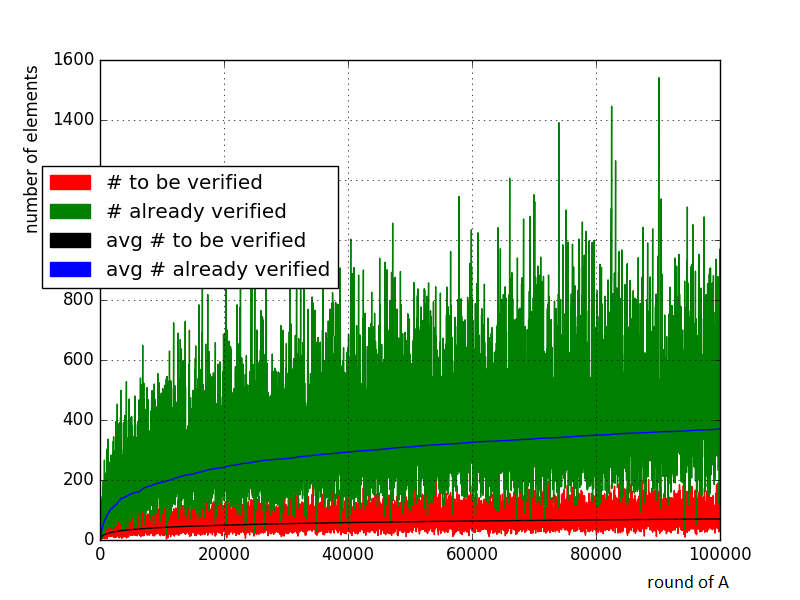
\includegraphics[width=9cm]{f_sum_build_spare_and_to_be_verified}
\caption[caption]{Sum building - first $10^5$ runds of $A$}
\label{fig:sumbuildsparever}
\end{figure}

Figure $\ref{fig:sumbuilddiff}$ depicts difference between $N_{max}$ and $N_{conf}$ for first consecutive rounds of $A$. Difference is fluctuating, with periodic ups and downs, but in general is relatively low in comparison to $r$ - for first $10^5$ round of $A$ it is $\leq$ 3500.

\begin{figure}[!ht]
\centering
\captionsetup{justification=centering}
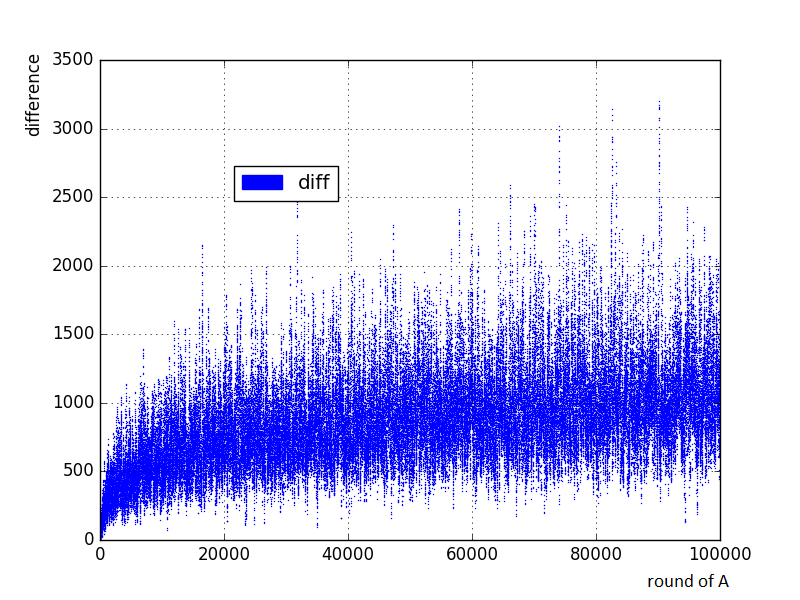
\includegraphics[width=9cm]{f_sumbuild_diff}
\caption[caption]{diff$(r)$ = $N_{max}(r)$ - $N_{conf}(r)$ where $r$ is a round of $A$; results for the first $10^5$ rounds of $A$}
\label{fig:sumbuilddiff}
\end{figure}

As a result of this work interesting integer sequence was submitted to OEIS database: OEIS A301776 \cite{A301776}. This sequence contains prime numbers $p$ with the property that all even numbers $n$ ($2 \textless n \leq 2p$) are the sum of two primes $\leq p$. Most probably OEIS A301776 is finite and has 7 terms only: $2, 3, 5, 7, 13, 19, 109$ - experiments were run for the first $10^5$  primes and no further terms were found. Figure $\ref{fig:sumbuild200}$ demonstrates effects of 200 first rounds of $A$ and visualises OEIS A301776. Red line depicts current $N_{conf}$, while green line - theoretical $N_{max}$. If lines are touching each other, we have a new term in OEIS A301776. \par

\begin{figure}[!ht]
\centering
\captionsetup{justification=centering}
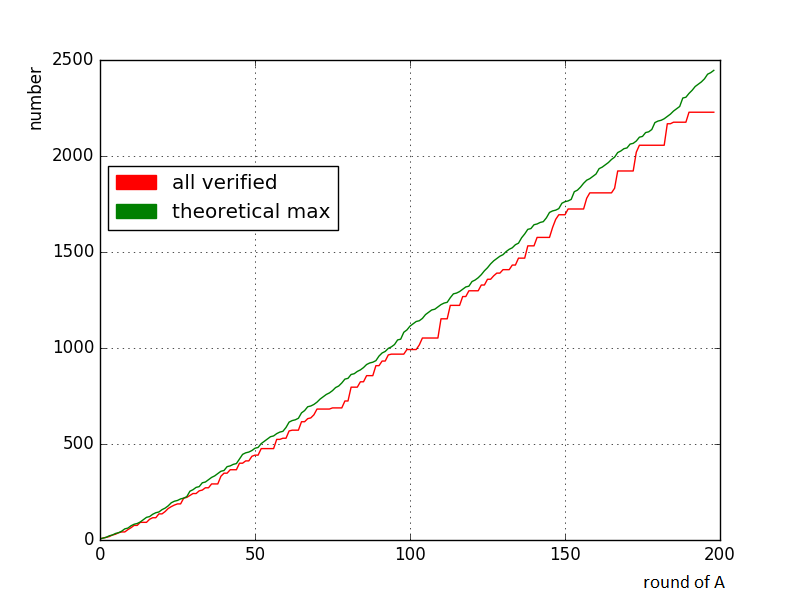
\includegraphics[width=9cm]{f_sumbuild_effectiveness_200}
\caption[caption]{$N_{max}$ (theoretical max) vs. $N_{conf}$ (all verified) - first 200 rounds of $A$}
\label{fig:sumbuild200}
\end{figure}

Figure $\ref{fig:sumbuildratioalrver}$ and Figure $\ref{fig:sumbuildratiotobever}$ show that there is correlation between $diff(r)$ and both $S_v(r)$ and $S_{nv}(r)$ (skipping cases from OEIS A301776 for which we have $0$ in denominator). After $10^5$ rounds arithmetical average of $\frac{diff(r)}{S_v(r)}$ equals 2.42635613793257 and arithmetical average of $\frac{diff(r)}{S_{nv}(r)}$ is 13.398628763226336. Figure $\ref{fig:sumbuildratioalrverdiff}$ and Figure $\ref{fig:sumbuildratiotobeverdiff}$ demonstrate that, in general, the bigger $r$, the smaller delta between two consecutive values of average difference, close to $0$.

\begin{figure}[!ht]
\centering
\captionsetup{justification=centering}
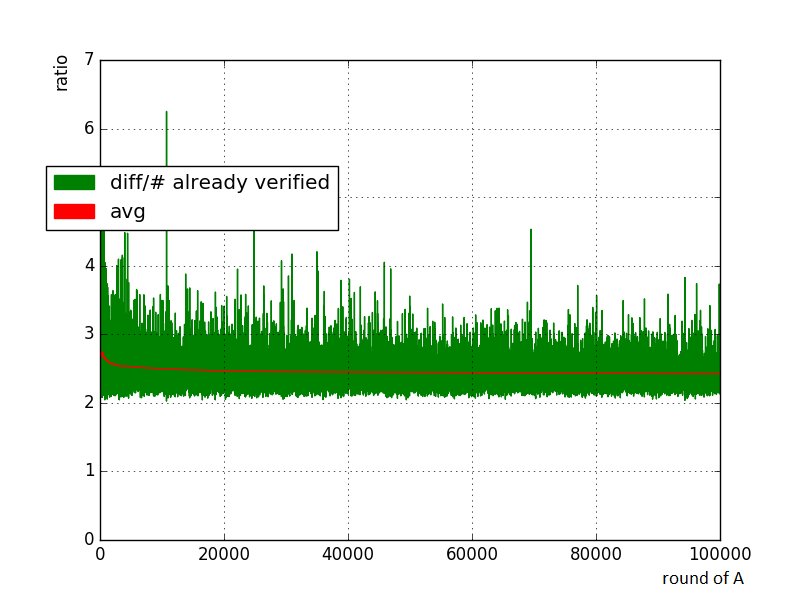
\includegraphics[width=9cm]{f_sumbuild_ratio_alr_ver}
\caption[caption]{Ratio $\frac{diff(r)}{S_v(r)}$, including average value (avg); results for the first $10^5$ rounds of $A$}
\label{fig:sumbuildratioalrver}
\end{figure}

\begin{figure}[!ht]
\centering
\captionsetup{justification=centering}
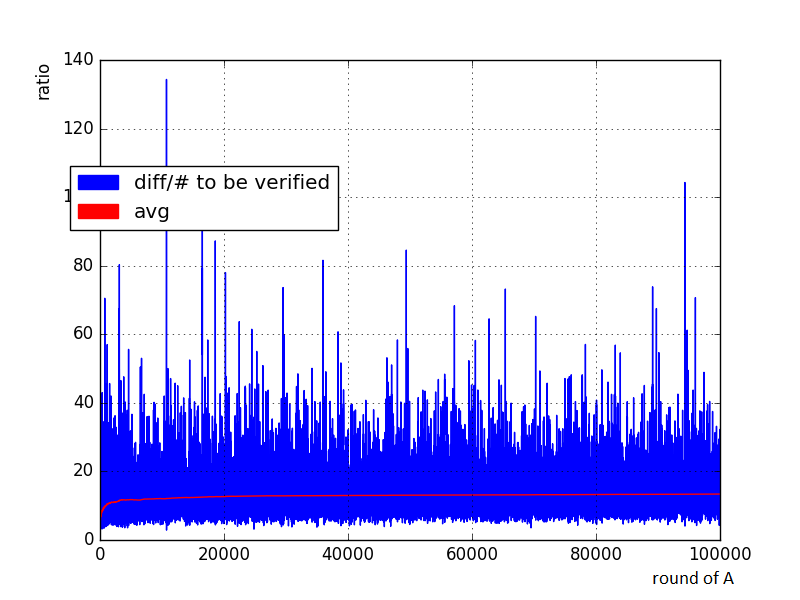
\includegraphics[width=9cm]{f_sumbuild_ratio_to_be_ver}
\caption[caption]{Ratio $\frac{diff(r)}{S_{nv}(r)}$, including average value (avg); results for the first $10^5$ rounds of $A$}
\label{fig:sumbuildratiotobever}
\end{figure}

\begin{figure}[!ht]
\centering
\captionsetup{justification=centering}
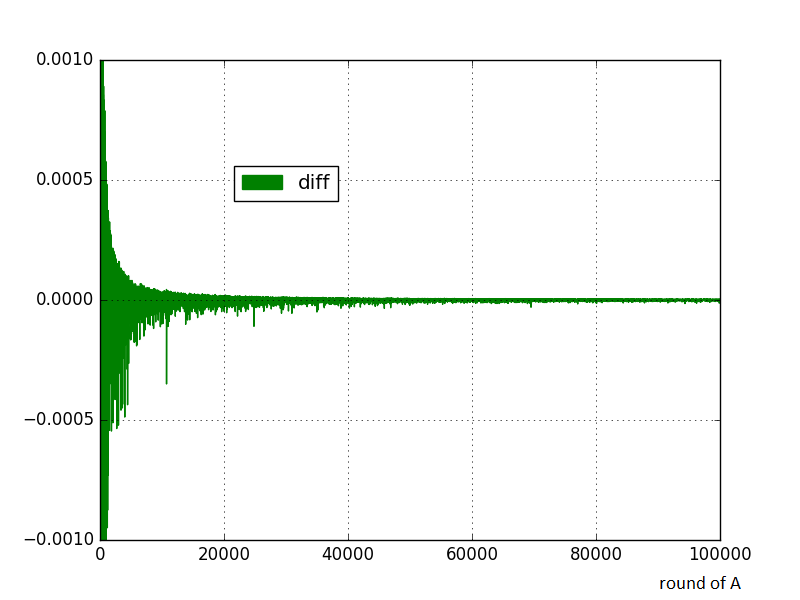
\includegraphics[width=9cm]{f_sumbuild_ratio_alr_ver_diff}
\caption[caption]{Consecutive difference in average of $\frac{diff(r)}{S_v(r)}$; results for the first $10^5$ rounds of $A$}
\label{fig:sumbuildratioalrverdiff}
\end{figure}

\begin{figure}[!ht]
\centering
\captionsetup{justification=centering}
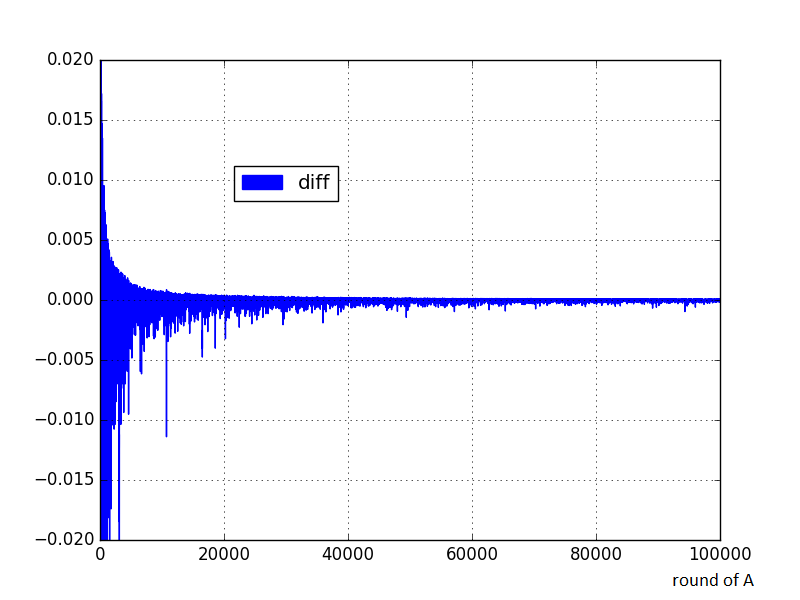
\includegraphics[width=9cm]{f_sumbuild_ratio_to_be_ver_diff}
\caption[caption]{Consecutive difference in average of $\frac{diff(r)}{S_{nv}(r)}$; results for the first $10^5$ rounds of $A$}
\label{fig:sumbuildratiotobeverdiff}
\end{figure}

\section{Summary}

Executed experiments provided data to formulate conjecture that there are only two even numbers $\textgreater 2$ (4 and 6) which have GP built from two identical primes: $4 = 2 + 2$, $6 = 3 + 3$ (and both numbers have no other partitions) and all greater even numbers $n$ have at least one partition $GSC(n, p_1, p_2)$, where $p_1 \neq p_2$ (2):

\begin{equation}
\displaystyle\mathop{\bigforall}_{x \textgreater 3, x \in \mathbb{N}} \displaystyle\mathop{\bigexists}_{p_1, p_2 \in \mathbb{P}, p_1 \neq p_2 } GSC (2x, p_1, p_2)
\end{equation}

In other words, if even number $n = 2p \textgreater 6$ (where p is prime), then exists a pair of primes $(p_1, p_2), p_1 \neq p_2$ that $GSC (n, p_1, p_2)$. Conjecture (2) says that all even numbers \textgreater 6 can be expressed as a sum of two different primes. \par
It still remains an open question if OEIS A301776 is finite or not. Executed experiments for the first $10^5$ primes confirmed that there are no other terms so far. Figure $\ref{fig:sumbuilddiff}$ gives a clue that there are cases for which we might be close to have a new term in the sequence (when difference is falling down, but never to $0$ for bigger primes) but then we have ups. Proving that there are other terms in OEIS A301776, especially proving that this sequence is infinite, would be a good base for a proof of $GSC$ - if sequence OEIS A301776 is infinite, then there is always a prime $p$ for which we can build all even numbers up to $2p$ using two primes $\leq p$.

\begin{thebibliography}{9}
\bibitem{goldbach1742}
  Christian Goldbach, 
  \emph{On the margin of a letter to Leonard Euler},
  1742.
\bibitem{oliveira2012}
  Tomás Oliveira e Silva,
  \emph{Goldbach conjecture verification.}
  http://sweet.ua.pt/tos/goldbach.html,
  2012.
\bibitem{oliveira2013}
  Tomás Oliveira e Silva, Siegfried Herzog, and Silvio Pardi, 
  \emph{Empirical verification of the even Goldbach conjecture and computation of prime gaps up to 4 $\times 10^{18}$.}, 
  Mathematics of Computation, vol. 83, no. 288, pp. 2033-2060, 
  July 2014 (published electronically on November 18, 2013.
\bibitem{A301776}
  OEIS Foundation Inc. (2018), The On-Line Encyclopedia of Integer Sequences, http://oeis.org/A301776. Prime numbers p with the property that all even numbers n (2 $\textless$ n $\leq$ 2p) are the sum of two primes $\leq$ p.
  
\end{thebibliography}

\end{document}
